\documentclass[12pt]{article}
\usepackage[utf8]{inputenc}
\usepackage{geometry}
\usepackage{graphicx}
\usepackage{hyperref}
\usepackage{amsmath}
\usepackage{amsfonts}
\usepackage{listings}
\usepackage{xcolor}
\usepackage{float}
\usepackage{longtable}
\usepackage{array}
\usepackage{tabularx}
\usepackage{booktabs}
\usepackage{caption}
\usepackage{url}
\usepackage{tikz}
\usetikzlibrary{matrix, shapes, arrows, positioning}
\usepackage[document]{ragged2e}
\usepackage{placeins}

\geometry{a4paper, margin=1in}

\title{
    {\Huge System Verification and Validation Plan} \\
    {\Large for} \\
    {\LARGE Angry Bird Alike} \\
    \vspace{0.5em}
    {\Large Author: Al Jubair Hossain} \\
    \vspace{0.5em}
    {\large March 31, 2024}
}
\date{}

\begin{document}

\maketitle

\newpage

\section*{Revision History}
\begin{tabular}{|l|l|p{10cm}|}
    \hline
    \textbf{Date} & \textbf{Version} & \textbf{Notes} \\
    \hline
    February 3, 2024 & 1.0 & Initial draft completed. \\\hline
    February 25, 2024 & 1.5 & Revised draft with updates to testing strategies and test cases while changing section 9. \\\hline
    March 31, 2024 & 2.0 & Revised draft with changes to adding right Physics and Math formulas , specific description and changes in sections of 3, 4, 4.1-4.6, 5, 5.1-5.2.2 , 6- changes to traceability matrix relating with SRS tests, 7 - Unit Tests and appendix. And corrected Author Name \\
    \hline
\end{tabular}

\newpage

\tableofcontents

\newpage

\section{Symbols, Abbreviations, and Acronyms}

\subsection{Symbols}
The following symbols are used in this document to represent physical quantities and their units, aligned with the conventions established in the Software Requirements Specification (SRS) for "Angry Birds Alike".

\begin{itemize}
    \item \(m\) - Meter (Unit of length, significant for distance calculations in simulations)
    \item \(kg\) - Kilogram (Unit of mass, crucial for force and momentum calculations)
    \item \(s\) - Second (Unit of time, used for time-stepping in physics simulations)
    \item \(m/s\) - Meter per Second (Unit of velocity, describing the speed of objects)
    \item \(m/s^2\) - Meter per Second Squared (Unit of acceleration, including gravity)
    \item \(N\) - Newton (Unit of force, applicable in simulations involving collisions)
    \item \(rad\) - Radian (Unit for angular measurements, used in trajectory angles)
\end{itemize}

\subsection{Abbreviations and Acronyms}
This document and the associated Software Requirements Specification (SRS) utilize the following abbreviations and acronyms to ensure clarity and concise communication:

\begin{itemize}
    \item SRS - Software Requirements Specification
    \item VnV - Verification and Validation
    \item GUI - Graphical User Interface
    \item UAT - User Acceptance Testing
    \item RK4 - Runge-Kutta 4th Order Method
    \item SI - International System of Units
    \item AB\_Sim - Angry Birds Alike Simulation
\end{itemize}

\subsection{Mathematical Notation}
Consistent with the SRS, this document employs standard mathematical notation for clarity in describing algorithms, models, and calculations. Scalars (e.g., mass \(m\), time \(t\)) are denoted in italics, whereas vectors (e.g., velocity \(\mathbf{v}\), force \(\mathbf{F}\)) are represented in boldface. Differential equations and formulas integral to the game's physics engine are presented in a manner that facilitates understanding of the underlying mechanisms and their implementation.

\section{General Information}

\subsection{Summary}
This document outlines the Verification and Validation (VnV) Plan for "Angry Birds Alike," focusing on ensuring the game meets its intended functional and non-functional requirements. Designed to be both educational and entertaining, "Angry Birds Alike" targets a broad audience range, from young students to adults, by integrating physics-based puzzles that require strategic thinking and an understanding of basic physics principles. The VnV plan provides a systematic approach to verifying and validating each aspect of the game to deliver a high-quality user experience.

\subsection{Objectives}
The primary objectives of this VnV plan include:
\begin{enumerate}
    \item \textbf{Alignment with SRS:} Ensuring that "Angry Birds Alike" adheres to all outlined functional and non-functional requirements as specified in the Software Requirements Specification (SRS).
    \item \textbf{User Satisfaction:} Confirming the game meets or exceeds user expectations in terms of gameplay, educational value, and overall performance, thereby establishing its appeal and utility to the intended audience.
    \item \textbf{Continuous Improvement:} Establishing a feedback loop based on user input and test results to facilitate ongoing refinement and enhancement of the game, aiming for perpetual improvement in quality and user engagement.
\end{enumerate}
Additionally, this plan recognizes constraints such as development timelines and resource availability, proposing a feasible approach to execution within these bounds.

\subsection{Relevant Documentation}
The VnV efforts for "Angry Birds Alike" are supported and informed by several key documents:
\begin{itemize}
    \item \textbf{Software Requirements Specification (SRS):} The foundational document detailing functional and non-functional requirements, serving as the primary reference for verification and validation activities.
    \item \textbf{Design Documentation:} Provides insight into the game's architectural design, including system components and their interactions, which are critical for understanding implementation strategies and testing integration.
    \item \textbf{User Manuals and Guides:} Essential for validating the user experience and usability of the game, these documents offer instructions and guidance for end-users.
    \item \textbf{Previous Version Release Notes and Documentation:} If applicable, these documents supply valuable historical context for issues, improvements, and user feedback, which can inform current VnV strategies.
\end{itemize}

\section{Integration of Requirements and Models from SRS}

This section aligns the VnV activities with the detailed requirements and models outlined in the Software Requirements Specification (SRS) for "Angry Birds Alike." It ensures that every aspect of the game's design and development is subjected to rigorous verification and validation against the SRS to ensure compliance with the intended functionality and quality standards.

\subsection{Theoretical Models}
The theoretical models described in the SRS form the basis for the game's physics engine and gameplay mechanics. Verification of these models will involve both analytical methods and empirical testing to ensure their correct implementation. The models include:

\begin{enumerate}
    \item \textbf{Projectile Motion Model (TM1):} Ensures that the trajectory of projectiles launched by the player accurately follows the principles of physics. The model takes into account initial velocity, angle of launch, and gravitational effects to simulate realistic motion.
    \item \textbf{Elastic Collision Model (TM2):} Validates the interactions between projectiles and targets, ensuring that collisions adhere to the principles of conservation of momentum and energy. This model is critical for the game's puzzle-solving mechanics, where players must strategically use the environment and obstacles to achieve objectives.
    \item \textbf{Gravity Model (TM3):} Verifies the consistent application of gravitational forces to all objects within the game environment, contributing to the realism and educational value of the game. This model affects not only projectile motion but also the stability and collapse of structures within the game.
\end{enumerate}

\subsection{Instance Models}
Instance models derived from the theoretical foundations provide specific scenarios and interactions to be tested within the game. These models translate abstract principles into concrete game mechanics and scenarios:

\begin{enumerate}
    \item \textbf{Trajectory Calculation (IM1):} This model involves the calculation of projectile paths based on player inputs and environmental factors. Verification will include testing for accuracy in trajectory prediction and the impact of variable inputs such as launch power and angle.
    \item \textbf{Collision Detection and Response (IM2):} Focuses on the game's ability to detect and respond to collisions between objects. Validation will ensure that the outcomes of collisions—such as the destruction of obstacles and the defeat of targets—are consistent with expected physics behaviors.
\end{enumerate}

\section{Plan}

This section provides a detailed outline of the Verification and Validation (VnV) strategy for "Angry Birds Alike." The plan is structured to ensure comprehensive coverage of all aspects of the game, from its core physics engine to the user interface, ensuring that the game meets all specified functional and non-functional requirements.

\subsection{Verification and Validation Team}
The VnV team is comprised of dedicated professionals with expertise in software testing, quality assurance, and user experience design. The team includes:

\begin{itemize}
    \item \textbf{VnV Lead (Al Jubair Hossain):} Oversees the entire VnV process, ensuring that the plan is executed effectively and aligns with the project's objectives.
    \item \textbf{Test Engineer (Al Jubair Hossain):} Responsible for designing, implementing, and executing test cases. Lead will analyze test results and document any defects or issues.
    \item \textbf{Quality Assurance Analyst (Al Jubair Hossain):} Focus on the broader aspects of game quality, including performance, usability, and compliance with standards. The lead will also manage feedback from user acceptance tests.
\end{itemize}

\subsection{SRS Verification Plan}
The Software Requirements Specification (SRS) document is the foundation of the VnV process. Verification of the SRS involves:

\begin{enumerate}
    \item \textbf{Peer Review:} Conducted by team members who were not involved in the original drafting of the SRS, to identify any ambiguities or inconsistencies.
    \item \textbf{Requirement Traceability Analysis:} A systematic review to ensure that each requirement is traceable through the subsequent phases of design, implementation, and testing.
\end{enumerate}

\subsection{Design Verification Plan}
The design documents are essential for understanding the game's architecture and implementation strategy. Verification includes:

\begin{enumerate}
    \item \textbf{Design Review Meetings:} Scheduled discussions among the development team to review and evaluate design decisions and their alignment with the SRS.
    \item \textbf{Static Analysis:} Utilizing automated tools to analyze design models for consistency, completeness, and structural integrity.
\end{enumerate}

\subsection{Implementation Verification Plan}
Ensuring that the game's implementation adheres to the design specifications and meets the stated requirements involves:

\begin{enumerate}
    \item \textbf{Unit Testing:} Testing individual components or units of the game in isolation to validate their correct behavior.
    \item \textbf{Integration Testing:} Assessing the interaction between integrated components to ensure they work together as intended.
    \item \textbf{System Testing:} Evaluating the complete and integrated game software to ensure it meets all specified requirements.
\end{enumerate}

\subsection{Automated Testing and Verification Tools}
To enhance efficiency and coverage, the following automated tools will be utilized:

\begin{itemize}
    \item \textbf{CPPCheck} (or equivalent): For executing unit tests, analyzing code and ensuring code integrity.
    \item \textbf{Catch2:} Reliable and light xunit testing tool which is preferred by many C++ Programmers.
    \item \textbf{Google Test:} Another tool for automated and unit testing.
\end{itemize}

\subsection{Software Validation Plan}
Validation focuses on ensuring the game meets the needs and expectations of its users. Key activities include:

\begin{enumerate}
    \item \textbf{User Acceptance Testing (UAT):} Engaging with a select group of end-users to validate the game in real-world usage scenarios.
    \item \textbf{Beta Testing:} Releasing the game to a broader audience to gather feedback on its performance, usability, and overall satisfaction.
    \item \textbf{Feedback Analysis:} Collecting and analyzing feedback from all testing activities to guide future improvements and enhancements.
\end{enumerate}

\section{System Test Description}

This section outlines the specific strategies for system testing "Angry Birds Alike," focusing on validating both functional and non-functional requirements as derived from the Software Requirements Specification (SRS). The tests are designed to ensure comprehensive coverage, verifying that the game operates as intended and meets the high expectations of its users.

\subsection{Tests for Functional Requirements}

Functional requirements encompass the essential behaviors and functionalities of the game. The tests in this category aim to verify that all game mechanics, physics simulations, and user interactions perform correctly.

\subsubsection{Projectile Trajectory and Impact Accuracy Test}
\begin{itemize}
    \item \textbf{Objective:} To verify that the trajectory of projectiles when launched at varying angles and velocities accurately follows the expected physics model, and that the impact on targets produces the correct game response.
    \item \textbf{Method:} Automated tests will simulate launches with a range of angles and power settings, comparing the actual trajectories and outcomes with the expected results based on physics calculations.
    \item \textbf{Expected Outcome:} Each projectile's path matches the theoretical trajectory, and impacts with targets result in appropriate reactions such as target displacement or destruction, consistent with the game's physics engine.
\end{itemize}

\subsubsection{Level Progression and Unlocking Mechanics Test}
\begin{itemize}
    \item \textbf{Objective:} Ensure that players can progress through levels upon meeting specific objectives, and that new levels unlock accordingly.
    \item \textbf{Method:} Manual and automated testing to complete levels under various conditions, observing the unlocking mechanism for subsequent levels.
    \item \textbf{Expected Outcome:} Upon completing a level's objectives, progress is correctly recorded, and the next level becomes accessible.
\end{itemize}

\subsection{Physics Engine Verification}
\subsubsection{Test Case: Projectile Motion Accuracy (TC1)}
\textbf{Objective:} Verify that the engine accurately calculates projectile trajectories within gravity.
\textbf{Method:} Compare simulated trajectories with theoretical predictions for various initial velocities and angles.
\textbf{Expected Outcome:} The simulated trajectories closely match theoretical calculations.

\subsubsection{Test Case: Collision Dynamics (TC2)}
\textbf{Objective:} Ensure collision outcomes adhere to conservation laws.
\textbf{Method:} Simulate collisions between objects of varying masses and velocities, assessing momentum and energy conservation.
\textbf{Expected Outcome:} Post-collision velocities and object states align with conservation principles.


\subsection{Tests for Non-functional Requirements}

Non-functional tests address the game's performance, usability, and overall quality, ensuring a satisfactory user experience beyond the core gameplay mechanics.

\subsubsection{Game Load Time and Performance Test}
\begin{itemize}
    \item \textbf{Objective:} Assess the game's performance, specifically focusing on load times and the smoothness of gameplay across different devices.
    \item \textbf{Method:} Utilizing performance testing tools to measure load times for the game and its levels, and monitoring the frame rate during gameplay under various conditions.
    \item \textbf{Expected Outcome:} Game load times do not exceed predefined thresholds, and the game maintains a stable frame rate, ensuring smooth gameplay without significant delays or visual stuttering.
\end{itemize}

\subsubsection{Usability and Accessibility Evaluation}
\begin{itemize}
    \item \textbf{Objective:} Confirm that the game is easily navigable and playable by users of all abilities, including those with accessibility needs.
    \item \textbf{Method:} User testing sessions involving players with a diverse range of abilities and familiarity with gaming, focusing on the intuitiveness of the interface and accessibility features.
    \item \textbf{Expected Outcome:} Users find the game interface to be intuitive and are able to play the game with minimal difficulty. Accessibility features support players with specific needs effectively.
\end{itemize}

\section{Traceability Matrix Integration}
This section integrates the Traceability Matrix from the Verification and Validation (VnV) Plan with the Software Requirements Specification (SRS), ensuring that each requirement specified in the SRS is directly linked to test cases and validation methods outlined in the VnV Plan. The integration provides a systematic approach to verify and validate that all SRS requirements are addressed and tested through the development lifecycle of "Angry Birds Alike."

\subsection{SRS Requirements to VnV Test Cases}
The following table outlines how SRS requirements correlate with VnV test cases, ensuring comprehensive coverage and validation of the game's functionalities and features.

\begin{longtable}{|p{0.2\linewidth}|p{0.6\linewidth}|p{0.2\linewidth}|}
\hline
\textbf{SRS Requirement ID} & \textbf{SRS Requirement Description} & \textbf{VnV Test Case ID(s)} \\
\hline
SRS-FR1 & User can control the angle and power of the projectile launch & VnV-TC1 \\\hline
SRS-FR2 & Projectiles exhibit realistic physics, including gravity and collision impacts & VnV-TC2 \\\hline
SRS-FR3 & Levels unlock sequentially after completing the previous level & VnV-TC3 \\\hline
SRS-FR4 & Users can restart a level at any time & VnV-TC4 \\\hline
SRS-FR5 & The game saves progress automatically & VnV-TC5 \\\hline
SRS-NFR1 & The game shall load within acceptable time limits on the target platform & VnV-TC6 \\\hline
SRS-NFR2 & The game shall maintain an acceptable frame rate on the target platform & VnV-TC7 \\\hline
SRS-NFR3 & Game controls shall be intuitive and accessible to players of all abilities & VnV-TC8 \\\hline
\hline
\end{longtable}

This matrix demonstrates the direct link between the "Angry Birds Alike" SRS requirements and the corresponding test cases outlined in the VnV Plan, ensuring that each functional and non-functional requirement is validated through targeted testing strategies.

\subsection{Specific Tools for C++ Game Development in VnV}
The VnV Plan for "Angry Birds Alike" employs specific tools tailored for C++ game development to facilitate testing, code analysis, and documentation:

\begin{itemize}
    \item \textbf{Static Code Analysis Tools:}
        \begin{itemize}
            \item \textbf{Cppcheck:} For automatic checks of C/C++ code to identify potential issues.
            \item \textbf{Clang Static Analyzer:} For deep analysis of C/C++ applications to identify bugs.
        \end{itemize}
    \item \textbf{Testing Frameworks:}
        \begin{itemize}
            \item \textbf{Catch2:} For unit testing with support for BDD-style test case description.
        \end{itemize}
    \item \textbf{Performance Testing Tools:}
        \begin{itemize}
            \item \textbf{Leaks:} For detecting memory management and threading bugs, and profiling programs.
            \item \textbf{Google Benchmark:} For benchmarking code snippets and gauging performance implications.
        \end{itemize}
    \item \textbf{Documentation Tools:}
        \begin{itemize}
            \item \textbf{Doxygen:} For generating software reference documentation from source files.
        \end{itemize}
\end{itemize}

These tools are critical for ensuring the "Angry Birds Alike" game meets its quality standards, offering a robust framework for verification and validation of the C++ codebase.

\section{Unit Test Description}

This section provides detailed descriptions of unit tests for the "Angry Birds Alike" game, ensuring individual components and modules function correctly as per the requirements specified in the Software Requirements Specification (SRS). These tests are crucial for identifying issues at the earliest stages of development.

\subsection{Unit Testing Scope}

Unit testing in "Angry Birds Alike" targets critical game components, ensuring their reliability and functionality. Key areas include:

\begin{itemize}
    \item Physics Engine: Verifying accuracy of physical simulations.
    \item User Interface (UI): Ensuring usability and responsiveness.
    \item Data Management: Validating correct data handling and storage.
    \item Game Logic: Confirming gameplay rules and mechanics operate as intended.
\end{itemize}

\subsection{Tests for Functional Requirements}

\subsubsection{Physics Engine - Projectile Motion}

\begin{itemize}
    \item \textbf{Test ID:} PE-01
    \item \textbf{Description:} Validate the projectile motion simulation for accuracy against predefined physics formulas.
    \item \textbf{Input:} Launch angle (30, 45, 60 degrees), velocity (10, 20, 30 m/s).
    \item \textbf{Expected Outcome:} The projectile follows a parabolic trajectory, with distances matching theoretical calculations.
    \item \textbf{Method:} Automated scripts compare simulated trajectories with theoretical outcomes.
\end{itemize}

\subsubsection{User Interface - Menu Navigation}

\begin{itemize}
    \item \textbf{Test ID:} UI-01
    \item \textbf{Description:} Ensure main menu navigation is intuitive and responsive.
    \item \textbf{Input:} User interactions with menu options.
    \item \textbf{Expected Outcome:} Seamless transition between menu screens without delays.
    \item \textbf{Method:} Manual testing by navigating through all menu options.
\end{itemize}

\subsection{Tests for Non-functional Requirements}

\subsubsection{Performance - Load Time}

\begin{itemize}
    \item \textbf{Test ID:} PF-01
    \item \textbf{Description:} Measure game load time to ensure it meets performance benchmarks.
    \item \textbf{Condition:} Testing performed on target platform specifications.
    \item \textbf{Expected Outcome:} Game loads within 5 seconds on the specified hardware.
    \item \textbf{Method:} Automated timing of game start-up to main menu access.
\end{itemize}

\subsubsection{Data Management - Progress Save}

\begin{itemize}
    \item \textbf{Test ID:} DM-01
    \item \textbf{Description:} Confirm that game progress is correctly saved and retrievable.
    \item \textbf{Input:} Simulated game progress.
    \item \textbf{Expected Outcome:} Game state is accurately saved and loaded upon restart.
    \item \textbf{Method:} Manual testing with restarts and checking for data persistence.
\end{itemize}

\subsection{Traceability Between Test Cases and Modules}

To ensure thorough validation of each module, a traceability matrix maps unit test cases to the specific modules they verify:

\begin{table}[H]
\centering
\begin{tabular}{|l|l|l|}
\hline
\textbf{Module} & \textbf{Functional Requirements} & \textbf{Test Case IDs} \\
\hline
Physics Engine & Projectile motion, Collision response, Gravity & TC1, TC2 \\\hline
User Interface & Intuitiveness, Accessibility & TC3, TC8 \\\hline
Game Mechanics & Level progression, Saving/Loading & TC4, TC5 \\\hline
Reset \& Performance & Load time, Frame rate stability & TC6, TC7 \\\hline
\hline
\end{tabular}
\caption{Traceability matrix mapping modules to functional requirements and test cases.}
\end{table}

This matrix ensures comprehensive coverage, with each module's key functionalities tested against both specific requirements and overall system performance and usability criteria.


Each test case is designed to rigorously verify the functionality and performance of "Angry Birds Alike" components, ensuring a robust and reliable gaming experience for users.

\subsection{Traceability and Test Coverage}
This matrix links SRS requirements, MG modules, and VnV test cases to ensure comprehensive coverage and coherence across documentation.


\begin{table}[H]
\centering
\begin{tabular}{|l|l|l|}
\hline
\textbf{SRS Requirement} & \textbf{MG Module} & \textbf{VnV Test Case} \\
\hline
IM1: Projectile Motion & M4: Physics Engine & TC1: Projectile Motion Accuracy \\
IM2: Collision Dynamics & M4: Physics Engine & TC2: Collision Dynamics \\
IM3: Gravity Effects & M4: Physics Engine & TC1: Gravity Effects Verification \\
\hline
\end{tabular}
\caption{Traceability Matrix linking SRS Requirements, MG Modules, and VnV Test Cases.}
\end{table}


\section{Exit Criteria}
Exit criteria define the conditions that must be met before concluding the verification and validation activities for "Angry Birds Alike." The completion of these activities ensures that the game meets the established quality standards and requirements. The exit criteria include:
\begin{itemize}
    \item Successful completion of all static and dynamic testing activities.
    \item All identified defects and issues are addressed and resolved.
    \item Code coverage meets or exceeds the defined threshold.
    \item User scenario testing and performance testing meet or exceed predefined acceptance criteria.
    \item Documentation is updated to reflect any changes made during the testing process.
    \item Formal approval from stakeholders or the quality assurance team is obtained.
\end{itemize}

\section{Responsibilities}
Responsibilities for verification and validation activities are distributed among the project team as follows:
\begin{itemize}
    \item \textbf{Developers:}
    \begin{itemize}
        \item Responsible for coding and addressing issues identified during code reviews.
        \item Conduct unit testing for individual software components.
    \end{itemize}
    \item \textbf{Testers:}
    \begin{itemize}
        \item Conduct integration testing and user scenario testing.
        \item Perform performance testing to assess the application's responsiveness and stability under load.
    \end{itemize}
    \item \textbf{Project Managers:}
    \begin{itemize}
        \item Oversee the entire verification and validation process to ensure adherence to project timelines and quality standards.
        \item Ensure that testing activities are conducted according to the schedule.
        \item Approve exit criteria for each testing phase to proceed to the next stages of development or release.
    \end{itemize}
\end{itemize}

\section{Tools and Resources}
The verification and validation process for "Angry Birds Alike" employs a selection of tools and resources tailored to support C++ development, ensuring thorough testing, efficient code review, and performance optimization. These tools facilitate various aspects of the testing process, from static analysis and unit testing to performance evaluation.

\subsection{Code Review Tools}
\begin{itemize}
    \item \textbf{GitHub Pull Requests:} Enables collaborative code reviews within a git repository, allowing developers to comment, suggest improvements, and approve changes, fostering high-quality code standards.
    \item \textbf{Phabricator:} A suite of open source tools for peer code review, it facilitates reviewing and auditing code. It integrates with Git, Mercurial, and SVN.
\end{itemize}

\subsection{Static Code Analysis Tools}
\begin{itemize}
    \item \textbf{Cppcheck:} A static analysis tool for C/C++ code, Cppcheck provides automatic checks for various code issues, including memory leaks, syntax errors, and undefined behavior, helping to improve code quality.
    \item \textbf{Clang Static Analyzer:} A source code analysis tool that provides a deep analysis of C/C++ applications, identifying bugs in the code such as buffer overflows, memory leaks, and logic errors.
\end{itemize}

\subsection{Testing Frameworks}
\begin{itemize}
    \item \textbf{Catch2:} As our primary testing framework, Catch2 offers a user-friendly approach for defining test cases and capturing test results. It supports Behavior-Driven Development (BDD) styles and provides detailed reports on test outcomes, facilitating efficient unit and integration testing practices.
\end{itemize}

\subsection{Performance Testing Tools}
\begin{itemize}
    \item \textbf{Leaks:} An instrumentation framework for checking  memory management, leaks and threading bugs, and profile programs in detail.
    \item \textbf{Google Benchmark:} A library for benchmarking code snippets, similar to unit tests. It's used for timing C++ code and gauging performance implications of code changes.
\end{itemize}

\subsection{Documentation Tools}
\begin{itemize}
    \item \textbf{Doxygen:} A documentation generator for writing software reference documentation. From a configured set of source files, it generates documentation in HTML, PDF, or LaTeX format. It is particularly useful for documenting the APIs of C++ projects.
    \item \textbf{Markdown with GitHub/GitLab:} Markdown files hosted in GitHub or GitLab repositories provide a simple and effective way to maintain project documentation, including installation guides, user manuals, and development notes, ensuring that the documentation is easily accessible and version-controlled alongside the code.
\end{itemize}

Leveraging these specific tools in the development and testing of "Angry Birds Alike" ensures that the project adheres to high standards of code quality

\section{Risks and Mitigation Strategies}
Identified risks and their corresponding mitigation strategies include:
\begin{enumerate}
    \item \textbf{Resource Constraints:} Limited resources may impact the scope or depth of testing activities.
    \begin{itemize}
        \item \textbf{Mitigation:} Prioritize testing activities based on risk and impact, focusing resources on critical areas first.
    \end{itemize}
    \item \textbf{Changing Requirements:} Modifications to game requirements can introduce delays or necessitate retesting.
    \begin{itemize}
        \item \textbf{Mitigation:} Implement an agile approach to accommodate changes efficiently, with clear communication channels for requirement updates.
    \end{itemize}
    \item \textbf{Tool Limitations:} The selected tools may not fully support the testing requirements or could introduce compatibility issues.
    \begin{itemize}
        \item \textbf{Mitigation:} Evaluate and select tools based on compatibility with the project's technology stack and testing needs. Regularly review and update toolsets.
    \end{itemize}
    \item \textbf{Integration Challenges:} Integrating individual components into a cohesive system may reveal issues not apparent during unit testing.
    \begin{itemize}
        \item \textbf{Mitigation:} Employ continuous integration practices and conduct integration testing early and often.
    \end{itemize}
    \item \textbf{Performance Bottlenecks:} Performance testing may identify critical bottlenecks affecting user experience.
    \begin{itemize}
        \item \textbf{Mitigation:} Analyze performance testing results to identify optimization opportunities. Implement code and infrastructure optimizations based on findings.
    \end{itemize}
\end{enumerate}
\textbf{Contingency Plans:}
\begin{itemize}
    \item Establish a rollback plan for critical releases to ensure system stability in case new changes introduce unforeseen issues.
    \item Regularly review and update risk assessments and mitigation strategies throughout the development lifecycle to adapt to new challenges.
    \item Develop contingency testing plans for critical scenarios, ensuring the application's core functionalities remain stable and reliable.
\end{itemize}

\section{Appendix}

\subsection{Appendix A: Symbolic Parameters}
Symbolic parameters used in the physics-based gaming application include:
\begin{itemize}
    \item \(v_0\): Initial velocity vector of the projectile.
    \item \(r_0\): Initial position vector of the projectile.
    \item \(F_{\text{net}}\): Net force vector acting on the projectile.
    \item \(t\): Time step size used in the simulation.
    \item \(a\): Acceleration vector of the projectile.
\end{itemize}
These parameters are crucial for simulating realistic physics behaviors in the game, allowing for dynamic interactions and enhancing gameplay experience.

\subsection{Appendix B: Usability Survey Questions}
A set of usability survey questions designed to gather user feedback on the game's interface, controls, and overall experience includes:
\begin{enumerate}
    \item How would you rate the overall user interface of the game in terms of clarity and ease of use? (1: Very Poor - 5: Excellent)
    \item Did you find the game controls intuitive for manipulating the initial conditions and parameters of the simulation? (Yes/No)
    \item How satisfied are you with the visual representation of physics-based interactions in the game? (Very Dissatisfied - Very Satisfied)
    \item Were the sound effects corresponding to key physics events effective and engaging? (Yes/No)
    \item Did you encounter any difficulties or confusion while adjusting launch angles, forces, or other physics parameters? If yes, please specify.
    \item How would you rate the responsiveness and smoothness of the gameplay in terms of graphics rendering and collision detection? (1: Very Poor - 5: Excellent)
    \item Would you like to see any additional features or improvements in future updates of the game? If yes, please provide suggestions.
    \item How likely are you to recommend this game to others? (1: Not Likely - 5: Very Likely)
    \item Please share any other comments, feedback, or concerns you have about the game.
\end{enumerate}

\subsection{Appendix C: Physics-Based Game Working Principle with Formulas}
The "Angry Birds Alike" game employs mathematical models and computational algorithms to simulate realistic physical interactions, focusing on projectile motion, collision dynamics, and numerical methods for these simulations.

\begin{itemize}
    \item \textbf{Projectile Launch:} Players set the initial conditions for projectile motion by adjusting the launch angle (\(\theta\)) and the force (\(F\)), determining the initial velocity (\(v_0 = \frac{F}{m}\)), where \(m\) is the projectile's mass.
    
    \item \textbf{Trajectory Calculation Using ODEs and RK4 Method:} The game calculates the projectile's trajectory by solving the motion equations, represented as Ordinary Differential Equations (ODEs), using the Runge-Kutta 4th order method (RK4). This method accurately predicts the projectile's path by calculating velocity and position increments at each time step. The RK4 method equations for a step are given by:
    
        \[
        k_1 = \Delta t \cdot f(t_n, y_n)
        \]
        \[
        k_2 = \Delta t \cdot f(t_n + \frac{1}{2}\Delta t, y_n + \frac{1}{2}k_1)
        \]
        \[
        k_3 = \Delta t \cdot f(t_n + \frac{1}{2}\Delta t, y_n + \frac{1}{2}k_2)
        \]
        \[
        k_4 = \Delta t \cdot f(t_n + \Delta t, y_n + k_3)
        \]
        \[
        y_{n+1} = y_n + \frac{1}{6}(k_1 + 2k_2 + 2k_3 + k_4)
        \]
        
        Where \(\Delta t\) is the time step, \(t_n\) and \(y_n\) are the current time and position, and \(f(t, y)\) represents the derivative of \(y\) with respect to \(t\). This process is repeated for both the horizontal (\(x\)) and vertical (\(y\)) components of motion to simulate the projectile's trajectory.
    
    \item \textbf{Distance Measurement Using RK4 Method:} The distance the projectile travels is calculated by integrating its horizontal velocity over time using the RK4 method, allowing accurate prediction of the landing point based on initial launch parameters.

    \item \textbf{Momentum and Elastic Collision:} Elastic collisions conserve both momentum and kinetic energy. For two colliding objects, momentum conservation is expressed as \(m_1v_{1,initial} + m_2v_{2,initial} = m_1v_{1,final} + m_2v_{2,final}\), and kinetic energy conservation as \(\frac{1}{2}m_1v_{1,initial}^2 + \frac{1}{2}m_2v_{2,initial}^2 = \frac{1}{2}m_1v_{1,final}^2 + \frac{1}{2}m_2v_{2,final}^2\).
    
    \item \textbf{Collision Detection:} Precise detection of collisions between the projectile and targets is based on the trajectory simulation, taking into account their shapes, sizes, and positions.
\end{itemize}

These physics principles and numerical methods ensure an engaging and educational gaming experience, demonstrating real-world physics through interactive gameplay in "Angry Birds Alike."

\section{Chart Diagram}
\textbf{Flowchart for "Angry Bird Alike" Gameplay}

\begin{figure}[!hb]
    \centering
    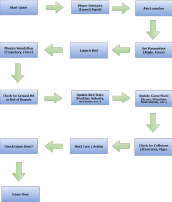
\includegraphics[width=0.5\linewidth]{Flowchartvnv.png}
    \caption{Flowchart diagram illustrating "Angry Birds Alike" gameplay mechanics and user interaction.}
    \label{fig:flowchart}
\end{figure}

\FloatBarrier
\section{Conclusion}
The revised Verification and Validation Plan for "Angry Birds Alike" incorporates specific enhancements and clarifications across various sections, including the integration of Catch2 for unit testing and an updated traceability matrix for improved clarity on how each module and functionality will be tested. These refinements ensure a robust framework for verifying and validating the game, supporting the development of a high-quality, engaging, and educational gaming experience.

\section{References}
\begin{enumerate}
    \item Butcher, J.C. (2008). "Numerical Methods for Ordinary Differential Equations". John Wiley \& Sons. This reference provides a comprehensive look at numerical methods, including the RK4 method, for solving ODEs, crucial for simulating realistic physics in games.
    \item Halliday, D., Resnick, R., \& Walker, J. (2014). "Fundamentals of Physics". John Wiley \& Sons. A foundational text covering physics principles, including mechanics and dynamics relevant to game physics simulation.
    \item Eberly, D. H. (2010). "Game Physics". Morgan Kaufmann. Explores the mathematical principles and theories underpinning modern game physics engines, including collision detection and response.
    \item Millington, I. (2007). "Game Physics Engine Development". CRC Press. A practical guide to developing physics engines for games, detailing both theory and implementation of physics simulations.
    \item Perry, William E. (2006). "Effective Methods for Software Testing." Provides strategies and techniques for conducting comprehensive software testing, relevant to verification and validation processes.
    \item Goldstein, H., Poole, C., \& Safko, J. (2002). "Classical Mechanics". Addison Wesley. Offers an in-depth exploration of classical mechanics, including detailed discussions on conservation laws and collision dynamics, essential for physics-based game development.
\end{enumerate}

\end{document}
